\documentclass[conference]{IEEEtran}
% \IEEEoverridecommandlockouts
% The preceding line is only needed to identify funding in the first footnote. If that is unneeded, please comment it out.
\usepackage{cite}
\usepackage{amsmath,amssymb,amsfonts}
\usepackage{algorithmic}
\usepackage{graphicx}
\usepackage{textcomp}
\usepackage{xcolor}
\def\BibTeX{{\rm B\kern-.05em{\sc i\kern-.025em b}\kern-.08em
    T\kern-.1667em\lower.7ex\hbox{E}\kern-.125emX}}
\begin{document}

\title{Term Project Progress Report 2\\
CSCI 562: Formal Specifications\\ }

\author{\IEEEauthorblockN{Scott Johnson}
\IEEEauthorblockA{\textit{Department of Computer Science} \\
\textit{University of North Dakota}\\
s.j.johnson@und.edu}
\and
\IEEEauthorblockN{Thomas Perez}
\IEEEauthorblockA{\textit{Department of Computer Science} \\
\textit{University of North Dakota}\\
thomas.perez@und.edu}
}

\maketitle

\begin{abstract}
This is a project progress report for the term project for CSCI 562: Formal Specifications. This is the second of such reports and will detail the informal specifications agreed upon and an updated class diagram for the TCAS-II system. It also includes information about expected future progress and participation of both members.
\end{abstract}

\section{Updated Class Diagram}
Figure \ref{fig:1} shows the updated class diagram for the TCAS-II system onboard an aircraft operated by the fictional ``JohnsonAir'' company. We specifically chose this name to distinguish between the craft under operation (i.e. the one in which the TCAS system under design is installed) and other crafts within the vicinity of this aircraft.

Some notes about this diagram:
\begin{itemize}
    \item Every \texttt{Aircraft} is uniquely identified by its transponder ident. This ident is a 4-digit code (using numbers 0-7) that can change. The Transponder within an aircraft handles the rotation of transponder ident codes. \texttt{JohnsonAircraft} specifically also have a ``tail'' identifier, which is a unique, unchanging identifier for the aircraft.
    \item Every \texttt{Aircraft} has a unique \texttt{Location} that identifies it, as well.
    \item While within range of detection of the TCAS-II system onboard the single \texttt{JohnsonAircraft}, other \texttt{Aircraft} are tracked by the TCAS-II system as \texttt{Target}s until an \texttt{Advisory} is issued based on whether they are within the time-to-collision of the \texttt{JohnsonAircraft}. A \texttt{Intruder} object replaces the \texttt{Target} once an \texttt{Advisory} is issued.
    \item One and only one \texttt{Advisory} can be active for a given \texttt{Intruder}.
    \item Each \texttt{Advisory} has an \texttt{AdvisoryType}, which is one of three values: \texttt{Traffic\_Advisory}, \texttt{Resolution\_Advisory}, or \texttt{Clear\_Of\_Conflict}.
    \item \texttt{Clear\_Of\_Conflict} is issued when one of the other \texttt{Advisory} objects is resolved, and lasts until the \texttt{Intruder} is replaced once more by a \texttt{Target}, at which point the \texttt{Advisory} is removed.
    \item ADS-B/out is required as per TSO C 91, TSO C 121, and TSO C 135 for the vast majority of airports because the airspace is becoming so dense. Class G (uncontrolled) airspace, where FAA restrictions are fairly limited and ADS-B/out is not required, is becoming increasingly rare. For this reason, it is assumed that all \texttt{Aircraft} are equipped with ADS-B/out and thus transmit their GPS coordinates (latitude and longitude).
    \item   The \texttt{DataMonitor} is a singleton object that monitors the transponder data for potential collisions and creates one or more \texttt{Advisory} objects. Each individual \texttt{Advisory} object will be associated with exactly one \texttt{Intruder} object. There will exist only a single \texttt{DataMonitor} within the entire system and it will be either on (enabled) or off (disabled, likely overridden).
    \item Mode-S transponders are required. If the transponder is of Mode-C, then the \texttt{DataMonitor} will be disabled and no \texttt{Advisory} objects will be issued. Since the system under design is a TCAS-II system, we assume that the equipped transponder of a \texttt{JohnsonAircraft} is always Mode-S.
    \item TCAS-II only provides vertical resolutions. Thus, the \texttt{targetVerticalSpeed} of an \texttt{Advisory} will be positive if the pilot is instructed to climb, negative if the pilot is instructed to descend, or 0.0 if the pilot is instructed to level off. If the pilot is instructed to maintain vertical speed, the \texttt{targetVerticalSpeed} will be set to the same value as the \texttt{verticalSpeed} of the \texttt{Aircraft}.
\end{itemize}

\begin{figure*}
    \centering
    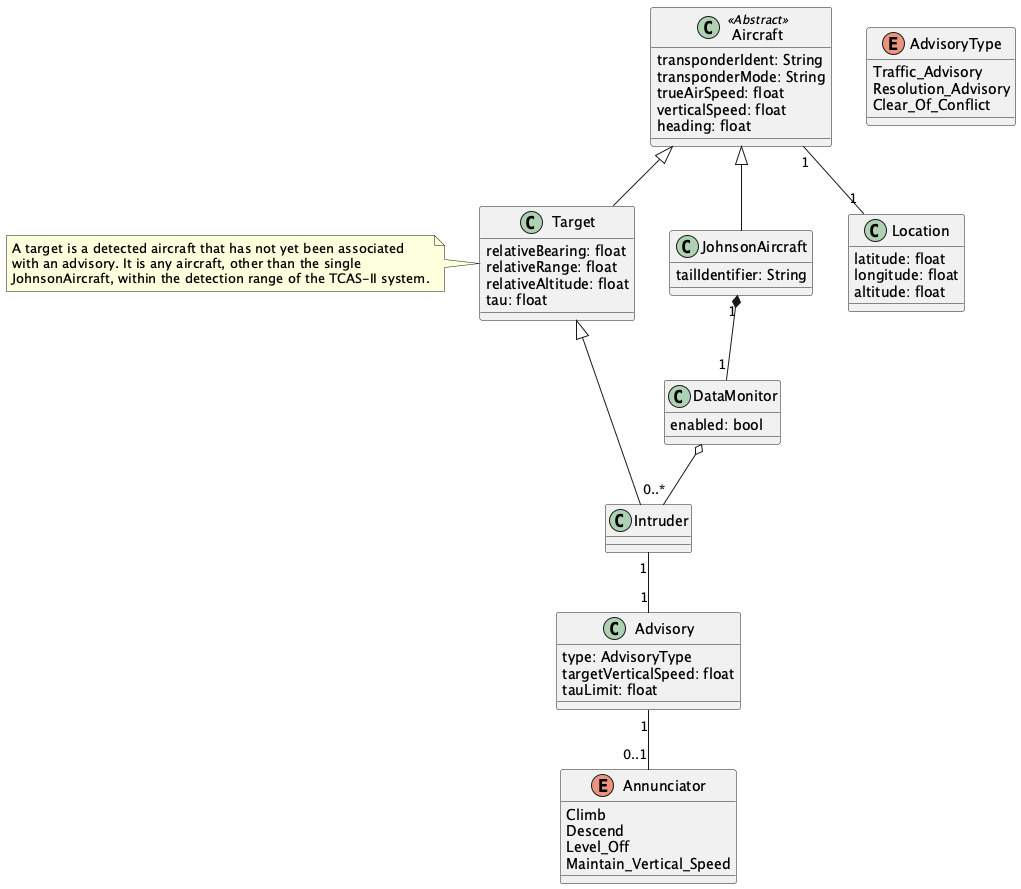
\includegraphics[width=0.8\textwidth]{classDiagram.png}
    \caption{Updated requirements class diagram for the TCAS-II system}
    \label{fig:1}
\end{figure*}

\section{Informal Specification}

The following is a summary of the information specifications we have thus developed. This is given in a textual format, similar to a W3C specification. Some of this is duplicated as part of the requirements class diagram, above.

\subsection{Introduction and General Notes}
The Traffic Collision Avoidance System II (TCAS-II) is an aircraft in-cockpit
system that is FAA mandated in specific use-cases \cite{1,2,3} to mitigate in-flight collisions. This is possible on aircraft equipped with a Mode-S transponder, with and without ADS-B/out. The system monitors surrounding in-flight traffic using these transponder signals. When conflicts or potential conflicts are detected, TCAS-II will provide the crew with a ``traffic advisory'' or a ``resolution advisory'' to maintain aircraft separation in a timely and collision-free manner, without abruptly maneuvering as smoothly as possible. An aggressive evasive maneuver, however, may have to be performed by the pilot flying in order to avoid a mid-air collision.\\

\subsection{Abbreviations}
The following abbreviations are used in this document:
\begin{itemize}
\item A/C (or a/c): Aircraft
\item ADS-B: Automatic Dependent Surveillance-Broadcast
\begin{itemize}
    \item ADS-B/in: FIS-B, and TIS-B. I,e., Flight Information Service (weather and forecasts), and Traffic Information Service. Almost every Aircraft currently supports ADS-B/in
    \item ADS-B/out: Sends GPS position, altitude, a/s, heading and aircraft ident. ADS-B/out does not replace the Mode-C transponder requirement; the aircraft must still have a Mode-C (or Mode-S)
\end{itemize}
\item Alt: Altitude
\item A/S, a/s: Horizontal airspeed
\item ATC: Air traffic control. They will be notified if an RA or TA is imminent. \cite{5} \cite{6} \cite{7}
\item CFR: Code of Federal Regulations
\item Deg: Bearing in degrees (0 - 359)
\item GPS: Global Positioning System
\item Ident: Aircraft identifier. 4 digit numeric code using the digits 0-7, inclusive.
\item MFD: Multifunction display
\item PF: Pilot flying
\item PNF: Pilot not flying
\item PFD: Primary flight display
\item RA: Resolution advisory
\item TA: Traffic advisory
\item VSI: Vertical speed indicator
\end{itemize}

\subsection{Inputs}
The following items are assumed to be inputs to the TCAS-II system:
\begin{itemize}
\item Mode-S transponder data
\item ADS-B signals
\item Target GPS position
\item Target Altitude
\item Target Vertical Speed
\item Target True Airspeed
\item Intruder Maneuver Information, Should a Resolution be necessary
\end{itemize}

\subsection{Outputs}
The TCAS-II system will output the following data:

\begin{itemize}
    \item Audible Signal indicating advisory type and Annunciation (if applicable)
    \item Visual Information, including RA visual commands, location of targets, icons indicating whether the target is climbing, descending, or leveled off.
\end{itemize}

\section{Schedule and Progress}
We are currently on schedule as per the Gantt chart indicated in progress report 1 \footnote{Please see progress report 1 resubmission, included with the submission of this report.}.

\subsection{Current Period Goals}
The following task(s) have been completed during this review period:
\begin{itemize}
    \item Project Breakdown and Gantt Chart (S. Johnson)
    \item Requirements UML Class Diagram (S. Johnson and T. Perez, jointly)
    \item Project Progress Report I Resubmission (S. Johnson and T. Perez, jointly)
    \item Project Progress Report II (S. Johnson and T. Perez, jointly)
    \item Define Textual Specification (T. Perez, who is our subject matter expert on Pilot Regulations)
    \item Definition of System Constraints (T. Perez)
    \item Informal Specification Write-up (S. Johnson)
\end{itemize}

We have weekly meetings scheduled for Thursday afternoons. Should you desire to participate in one of these meetings, we ask you to email us to verify we haven't rescheduled it, but otherwise, you are welcome at the meeting.

\subsection{Next Period Goals}
We intend to complete the following tasks for the next review period:

\begin{itemize}
    \item Selection of formal notation and tool (S. Johnson, T. Perez, jointly)
    \item First set of formal constraints (S. Johnson and T. Perez, jointly)
    \item Mapping of classes to schemas (S. Johnson, T. Perez, jointly)
    \item Division of system into subsystems for parallel work (S. Johnson)
\end{itemize}

\subsection{Issues and Blockers}
\begin{itemize}
    \item Papyrus was tried as a UML tool, but the design interface was non-intuitive. We used PlantUML, with VS Code integrations, to design the UML diagrams.
    \item The tool being used to track the project is Monday, but our subscription trial has run out. We may look into using something else, such as Linear, Notion, or some other tool, to maintain the Gantt chart. Monday is relatively expensive, and somewhat overkill for this project. We could use some advice on another tool that the University has a subscription to.
    \item S. Johnson is on travel from Mar 21-Mar 30 and again from April 20-24. He should have access to email during the second of these trips, but during the first, internet access will be spotty at best.
\end{itemize}

\begin{thebibliography}{00}
\bibitem{1}
U.S. Federal Aviation Administration,
\textit{14 C.F.R. Part-91 — General Operating and Flight Rules},
Code of Federal Regulations.

\bibitem{2}
U.S. Federal Aviation Administration,
\textit{14 C.F.R. Part-121 — Operating Requirements: Domestic, Flag, and Supplemental Operations},
Code of Federal Regulations.

\bibitem{3}
U.S. Federal Aviation Administration,
\textit{14 C.F.R. Part-135 — Operating Requirements: Commuter and On-Demand Operations},
Code of Federal Regulations.

\bibitem{4}
U.S. Federal Aviation Administration,
\textit{14 C.F.R. Part-71 — Designation of Class A, B, C, D, and E Airspace Areas; Air Traffic Service Routes; and Reporting Points, Code of Federal Regulations},
Code of Federal Regulations.

\bibitem{5}
U.S. Federal Aviation Administration,
\textit{14 C.F.R. Part-91.123 — General Operating and Flight Rules},
Code of Federal Regulations.

\bibitem{6}
U.S. Federal Aviation Administration,
\textit{14 C.F.R. Part-121.356 — Operating Requirements: Domestic, Flag, and Supplemental Operations},
Code of Federal Regulations.

\bibitem{7}
U.S. Federal Aviation Administration,
\textit{14 C.F.R. Part-135.19 and  Part-135.180 — Operating Requirements: Commuter and On-Demand Operations},
Code of Federal Regulations.

\end{thebibliography}
\end{document}
